%% V0.1
%% by Luis Batista, luisfelipew@gmail.com
%% This is a template for Udacity projects using IEEEtran.cls

\documentclass[10pt,journal,compsoc]{IEEEtran}

\usepackage[pdftex]{graphicx}    
\usepackage{cite}
\usepackage[table,xcdraw]{xcolor}
\usepackage{amssymb}
\usepackage{float}
\usepackage{caption}
\usepackage{subcaption}


\hyphenation{op-tical net-works semi-conduc-tor}
\graphicspath{{img/}}


\begin{document}

\title{Project: Map My World Robot}

\author{Luis F. W. Batista}

\markboth{SLAM project, Robotics Nanodegree Program, Udacity}%
{}
\IEEEtitleabstractindextext{%
\begin{abstract}
This paper presents and discusses the topic of Simultaneous Localization and Mapping (SLAM). Using ROS and Gazebo to simulate a customized robot equipped with an RGB-D camera and a Laser scanner, the Real-time Appearance-Based Mapping (RTAB-Map) implementation is used to generate a 2D occupancy grid map for two different environments. The produced maps and point clouds visually resemble the appearance of the original maps, and several loop-closures are detected when the robot is
passing by the same location.
\end{abstract}

\begin{IEEEkeywords}
Robot, IEEEtran, Udacity, \LaTeX, Mapping, ROS, Gazebo, SLAM.
\end{IEEEkeywords}}


\maketitle
\IEEEdisplaynontitleabstractindextext
\IEEEpeerreviewmaketitle
\section{Introduction}

\IEEEPARstart{I}{n} order for a robot to become fully autonomous, it is crucial to have the capability to perceive the environment and be able to locate itself within it. Those common tasks are known as Mapping and Localization. Simultaneous Localization and Mapping (SLAM), as the name indicates, is a technique capable of solving both the localization and mapping problems at the same time. It is accomplished during iterative cycles, using data collected from sensors.

In this project, SLAM is tested in two different simulated maps using ROS and Gazebo. The first environment, referred to as Kitchen and Dining World, is already available in Gazebo. The second map is a new environment created from scratch and referred to as My World.

To generate sensor data, a robot equipped with an RGB-D camera and 2D Lidar sensor is teleoperated in both simulated worlds.


\section{Background}

Localization and Mapping are extremely important for autonomous robots. In the localization problem, the robot is provided with the map of the environment and must estimate its pose. In the Mapping problem, the pose of the robot is known and it must create a map of its surroundings.

In many applications, the robot does not have a precise estimation of its position, neither the map of an unexplored area. In those situations, Simultaneous Localization And Mapping (SLAM) must be accomplished using only on the sensor data and the robot's own movements.

The interdependency of the two different problems makes SLAM very challenging. It is often considered as the Chicken or Egg type of problem. The map is needed for localization and the robot's pose is needed for mapping. Therefore, the accuracy of the map depends on the accuracy of the localization and vice versa.

SLAM can be separated into two forms: Full SLAM and Online SLAM. The first estimates map and the entire trajectory utilizing all the measurements and controls. The second only uses its current measurements and motion to estimate the map and the instantaneous poses.


\subsection{FastSLAM}

The FastSLAM algorithm solves the SLAM Problem using a particle filter approach to estimate a posterior over the trajectory. The predicted pose is then used for mapping, where a low dimensional Extended Kalman Filter is used to solve independent features of the map.

Three instances of the algorithm exists: FastSLAM 1.0, FastSLAM 2.0 AND Grid-based FastSLAM. Since the FastSLAM uses a particle filter approach to solve SLAM problems, it is a powerful algorithm capable of solving both the Full SLAM and Online SLAM problems.

\subsection{GraphSLAM}
GraphSLAM is an algorithm that solves the Full SLAM problem. As the name suggests, it uses graphs to represent the robot poses and map features that are tied together using motion and measurement constraints. As the robot moves around, several nodes are added updating the graph representation.

The algorithm can be separated in front-end and back-end. The front-end is  dependent on the application and the robot model, as it receives odometry and sensor measurements and is responsible for the data association problem. The back-end receives a complete graph with all the constraints and outputs the most probable configuration of robot poses and map features. It is responsible to optimize the representation using the maximum likelihood estimation to find the representation with the smallest error.

RealTime Appearance-Based Mapping (RTAB-Map) is one approach for implementing GraphSLAM. It uses data collected from vision sensors to localize the robot and map the environment. A process called loop closure is used to improve the accuracy of the results by determining whether the robot has seen a location before.

As the map expands and the number of images increases the loop closure complexity increases linearly. The algorithm is optimized for large-scale and long-term SLAM by using multiple strategies to allow for loop closure to be done in real-time, the result can be obtained before the next camera image is acquired.

This project uses the implementation of  RTAB-Map integrated with ROS and Gazebo to perform the SLAM task.





\section{Scene and robot configuration}
To perform SLAM, a robot was teleoperated in two different simulated environments. The data generated by the sensors are used by the RTAB-Map to generate the estimated map of the scene.

\subsection{World Scene}

Two simulated worlds were used. The first referred to as the Kitchen and Dining World is provided in Gazebo and used as a benchmark. It is shown on Figure \ref{fig:kitchen-dining-world}.

\begin{figure}[H]
  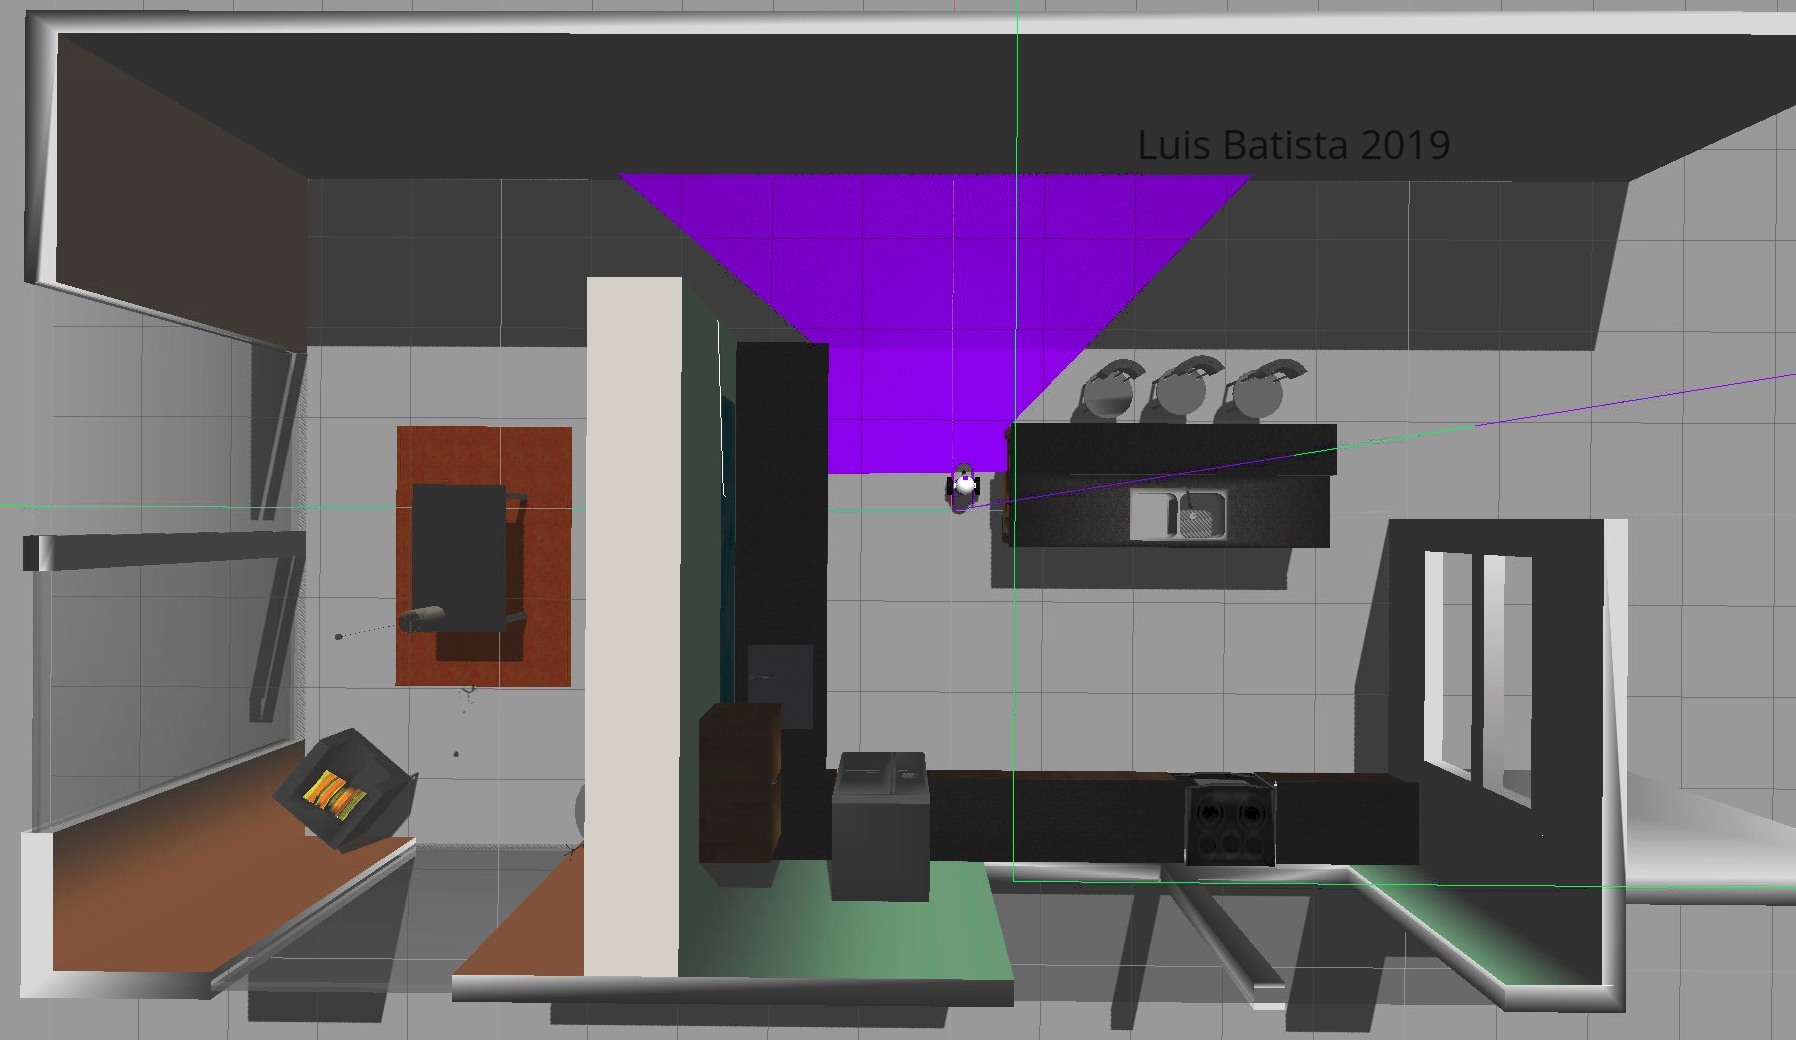
\includegraphics[width=\linewidth]{kd_world.png}
  \caption{Kitchen and Dining World}
  \label{fig:kitchen-dining-world}
\end{figure}

The second world, referred to as My World, was created from scratch using Gazebo. The Building Editor allows using a real floor plant image as a template. Basic features such as walls, doors, and windows can be easily added respecting a configurable scale.  
Several unique elements were placed around the room in order to improve the results of data associations used in the loop closure process of the SLAM algorithm. The result is shown in Figure \ref{fig:my-world}.

\begin{figure}[H]
  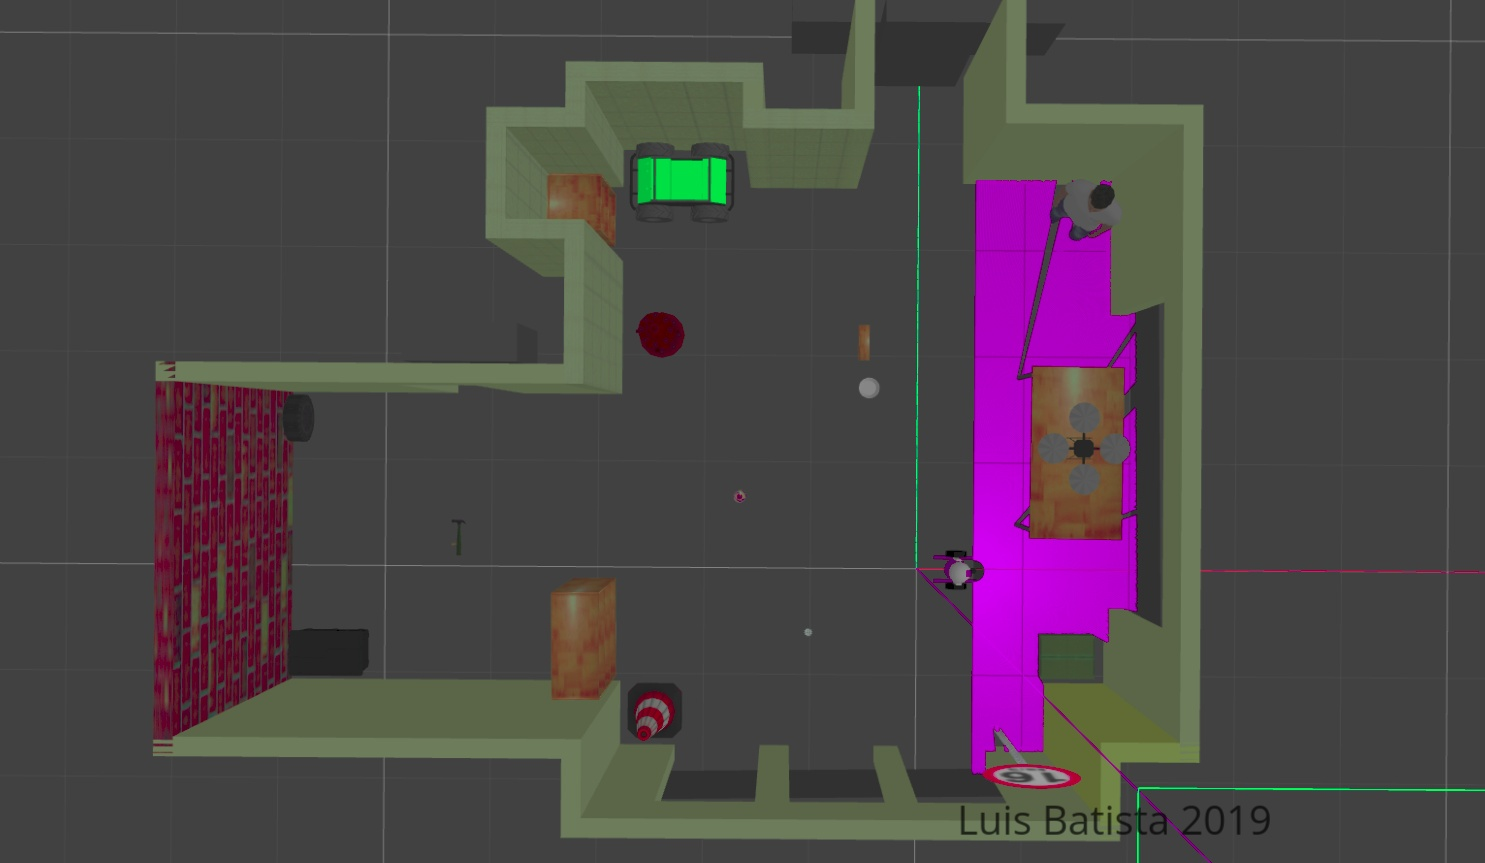
\includegraphics[width=\linewidth]{my_world.png}
  \caption{My World}
  \label{fig:my-world}
\end{figure}


\subsection{Robot Model}

The robot model, shown in Figure \ref{fig:robot-model}, has a moving a base with two actuators, an RGB-D camera, and a laser sensor. It was based on the robot developed for the previous localization project. The main change was the addition of an RGB-D camera used to provide the depth information and create a point cloud of the environment.

\begin{figure}[H]
  \centering
  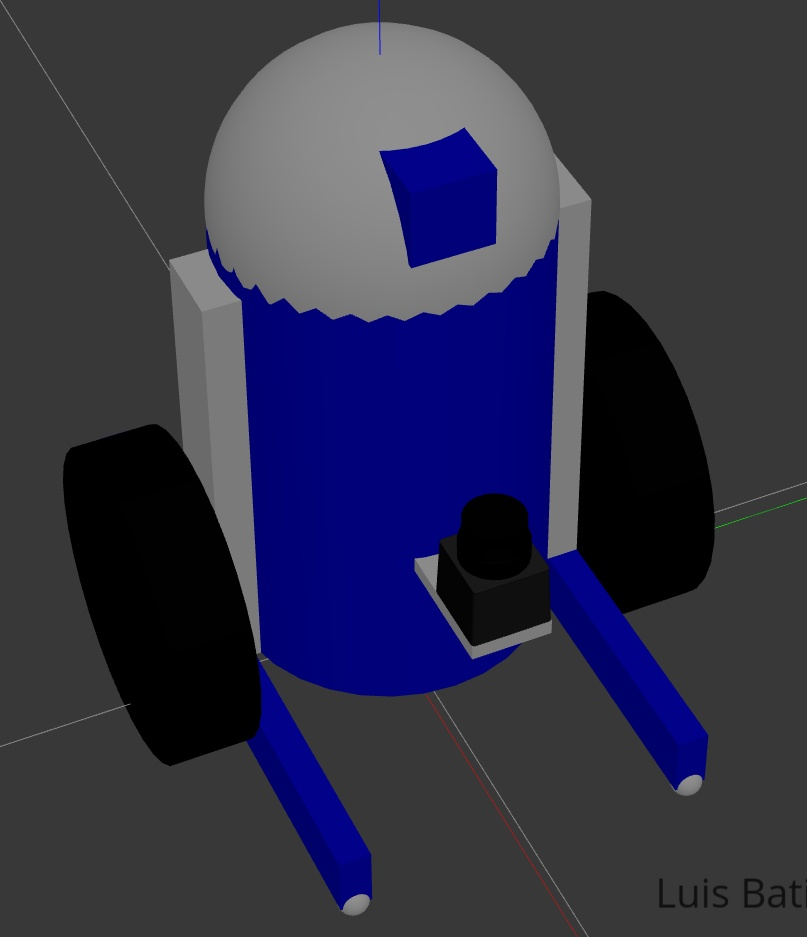
\includegraphics[width=.5\linewidth]{robot_model.png}
  \caption{Robot Model}
  \label{fig:robot-model}
\end{figure}

In order to calculate the robot position based on sensor data, they must be properly linked together to allow correct correlation. Figure \ref{fig:robot-tf-tree} shows the transformation tree links of the robot.

\begin{figure}[H]
  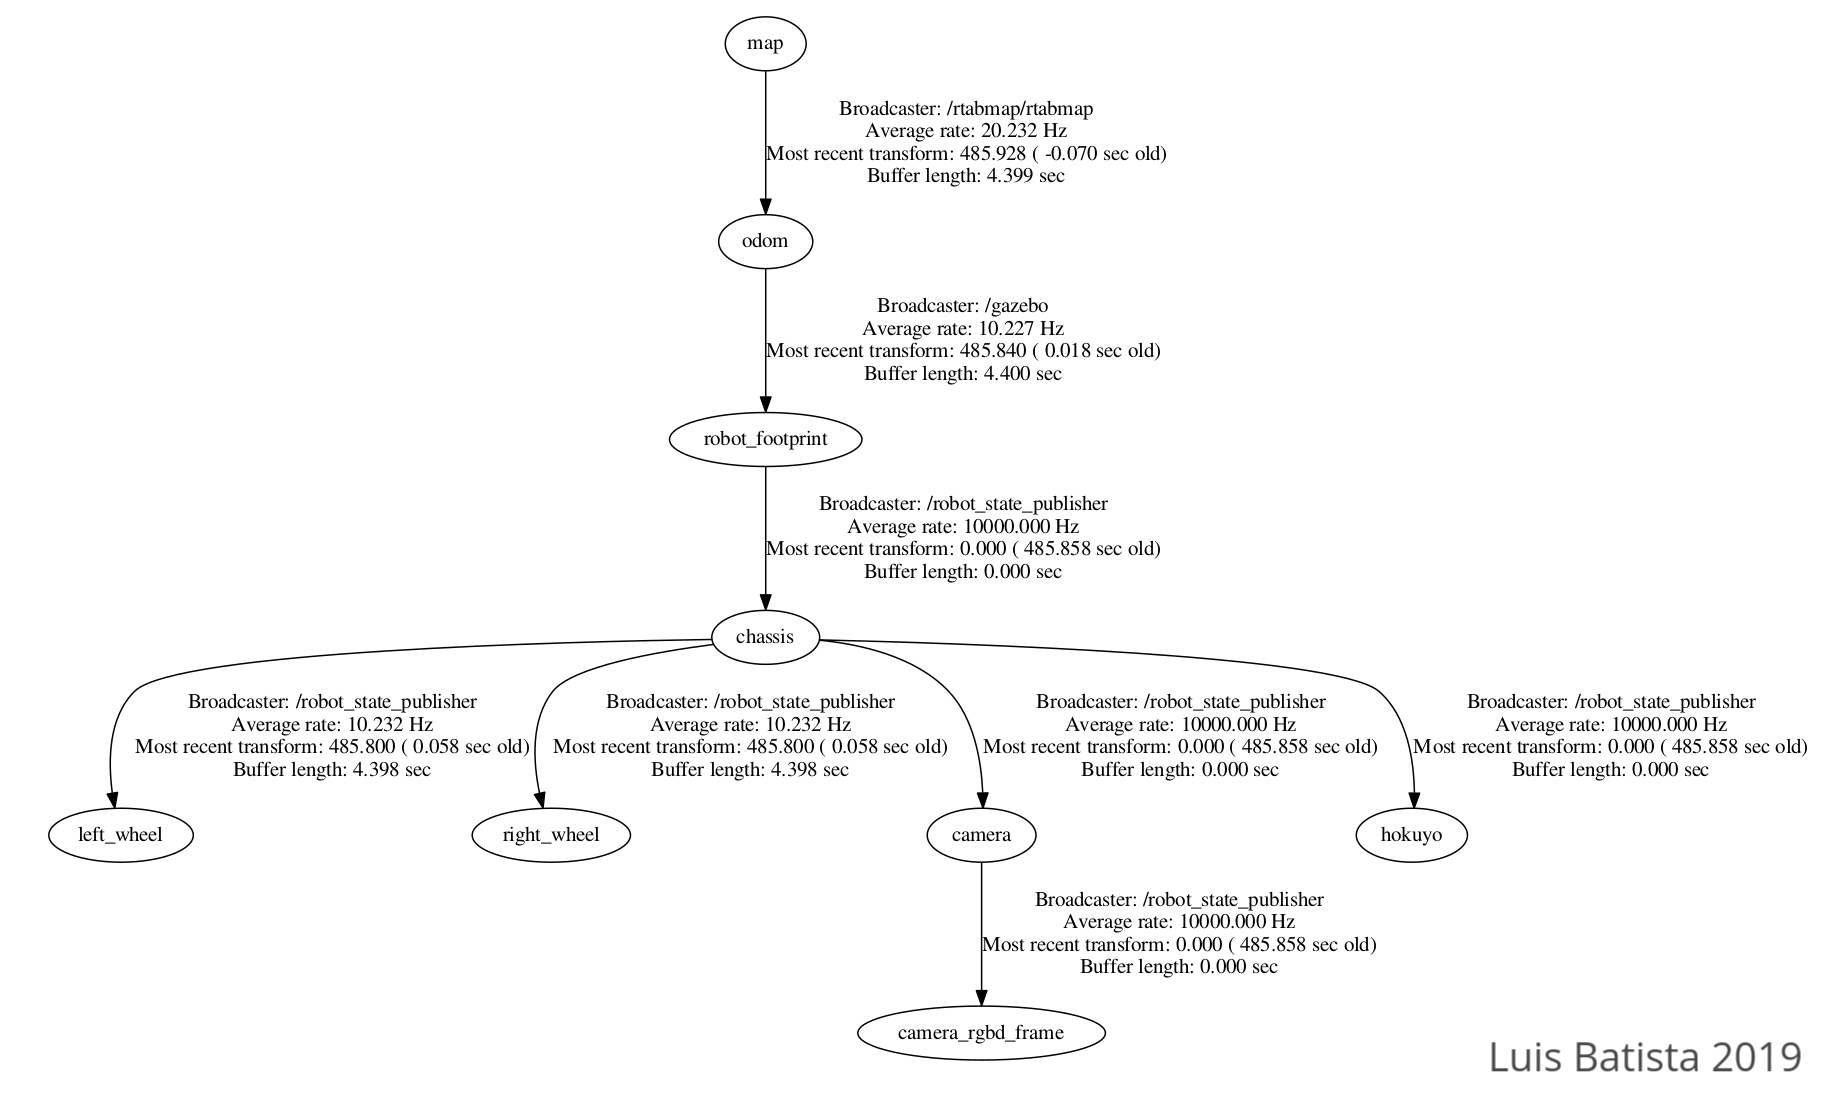
\includegraphics[width=\linewidth]{robot_tf_tree.png}
  \caption{Robot TF Tree}
  \label{fig:robot-tf-tree}
\end{figure}


\section{Results}


The generated map can be visually inspected using the database file generated by the RTAB-Map. The 2D map for both Worlds, including the robot's trajectory, has good fidelity comparing with the original map. The 2D map, including the robot's trajectory, for the Kitchen and Dining, can be seen in Figure \ref{fig:2d-map-kd}. Figure \ref{fig:2d-man-mw} shows the result for the My World environment.

\begin{figure}[H]
  \centering
  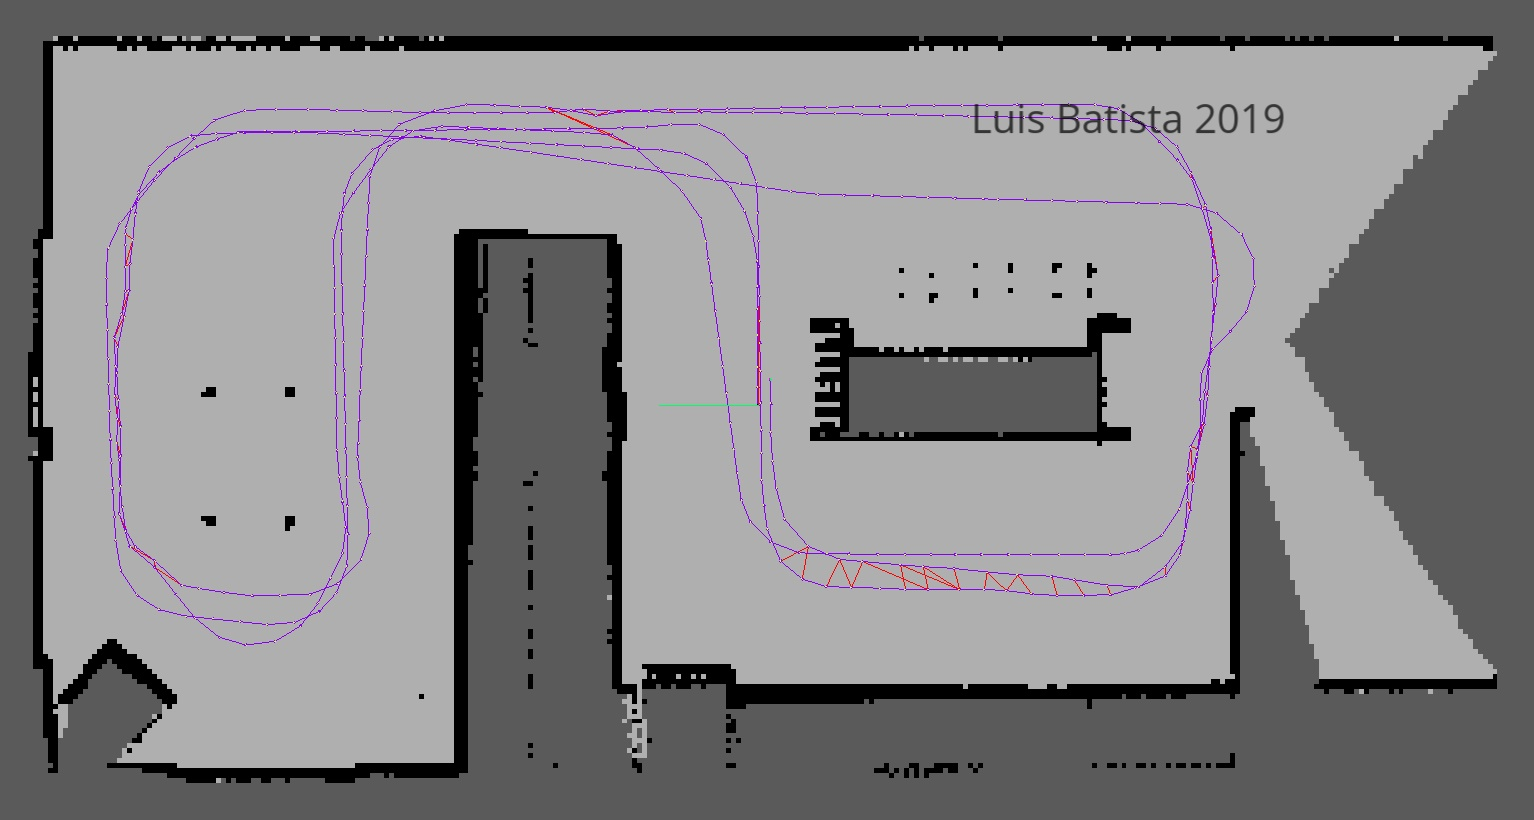
\includegraphics[width=.9\linewidth]{kd_world_2d.png}
  \caption{2D map - Kitchen and Dining World}
  \label{fig:2d-map-kd}
\end{figure}

\begin{figure}[H]
  \centering
  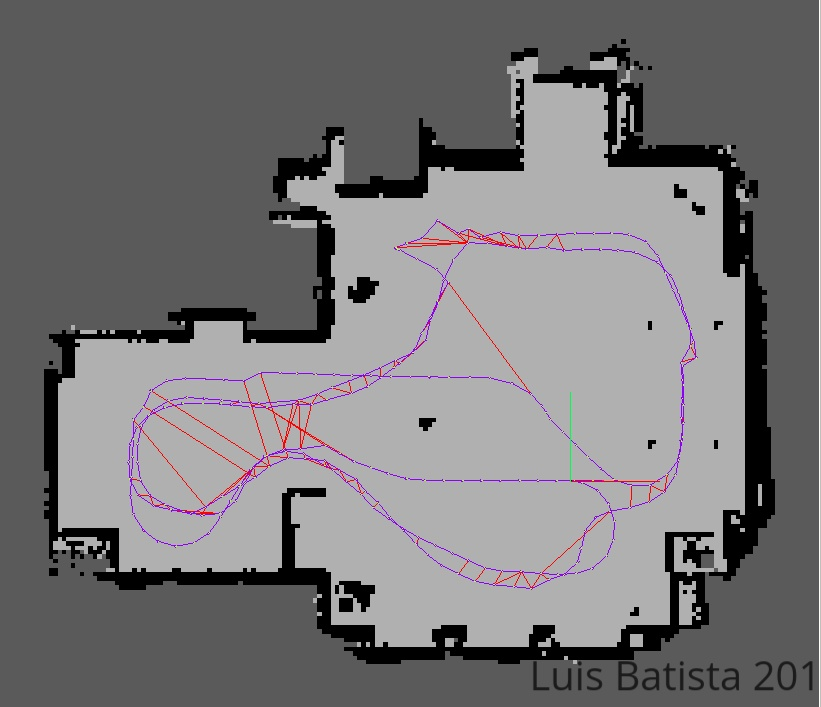
\includegraphics[width=.7\linewidth]{my_world_2d.png}
  \caption{2D map - My World}
  \label{fig:2d-man-mw}
\end{figure}

The map is calculated based on the data generated from the Laser scans. To address the uncertainty caused by the sensors noise, an algorithm known as Occupancy Grid Mapping is utilized. The map is represented as an evenly spaced field of values that represent the presence of an obstacle at that location in the environment.

Since it is based in a 2D Laser, only the obstacles located at the same height as the sensor is displayed. Figure \ref{fig:kd-og} shows the results for the Kitchen and Dining World, while Figure \ref{fig:my-og} shows the results for the My World environment.

\begin{figure}[H]
  \centering
  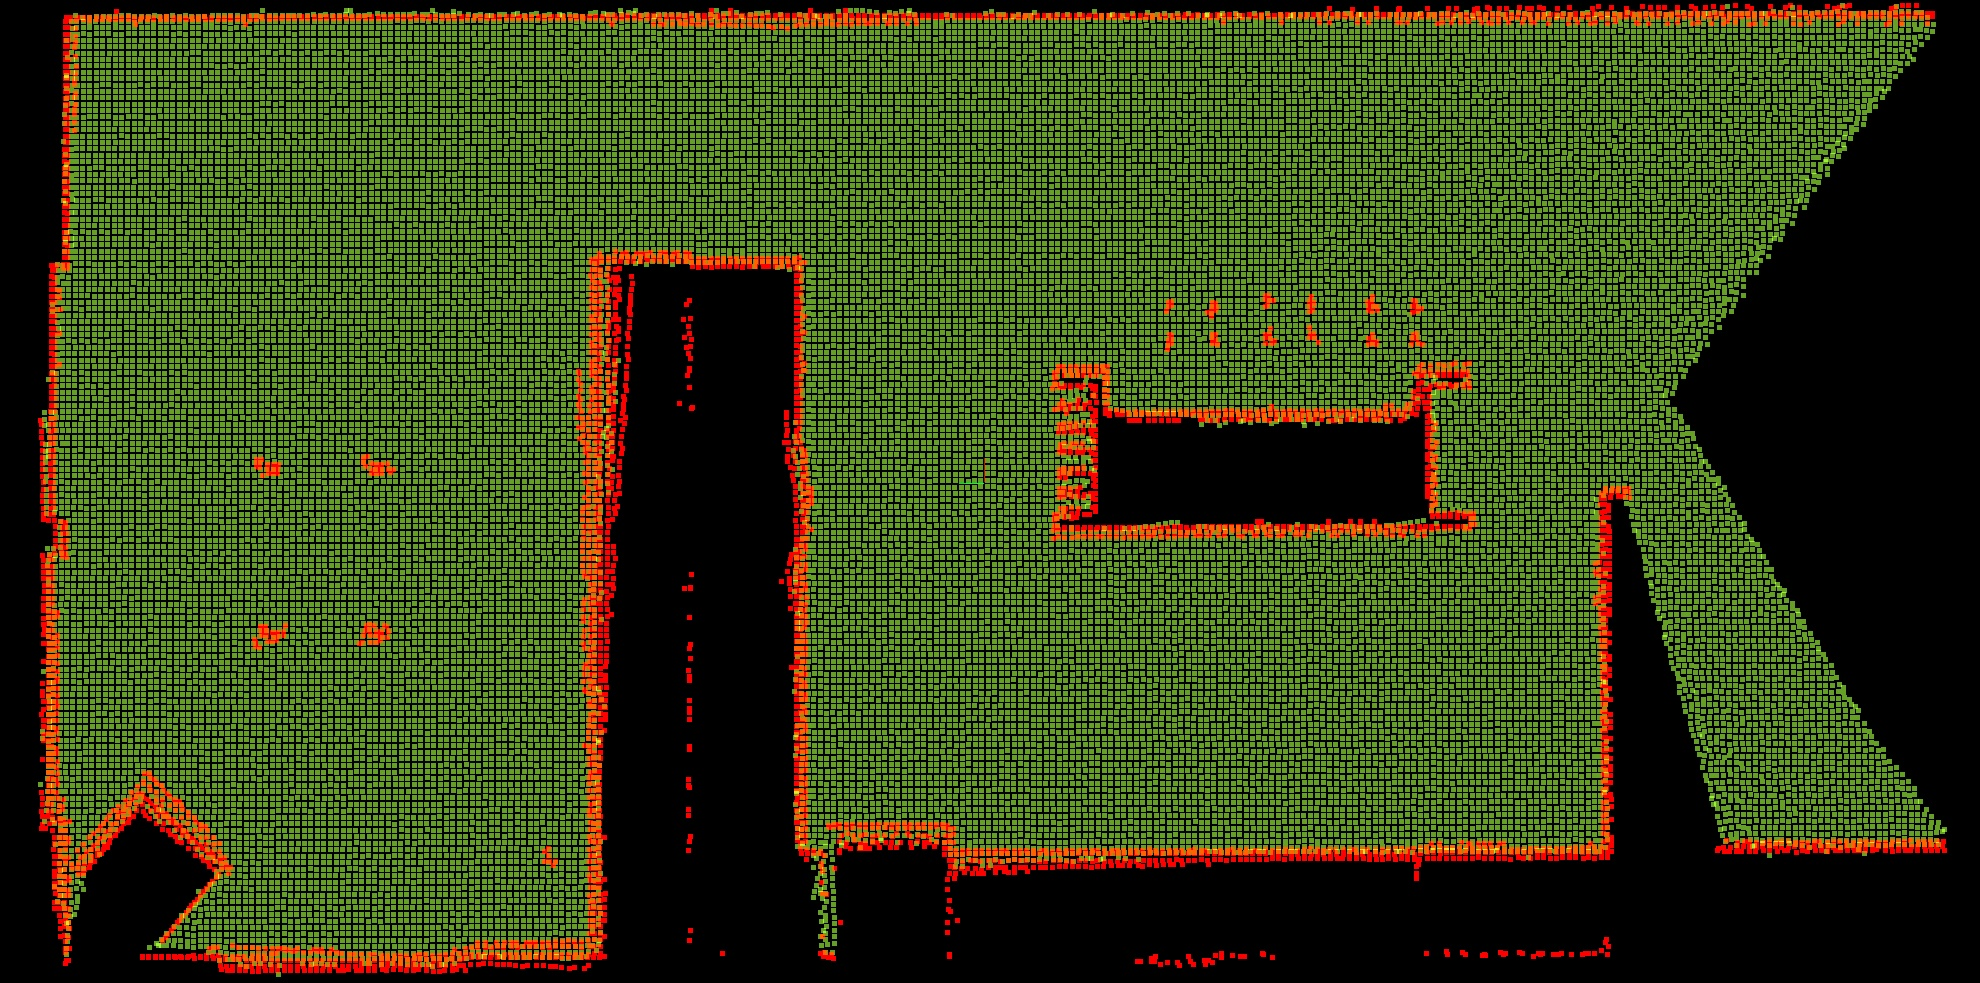
\includegraphics[width=.9\linewidth]{kd_world_og.png}
  \caption{Occupancy grid - Kitchen and Dining World}
  \label{fig:kd-og}
\end{figure}%

\begin{figure}[H]
  \centering
  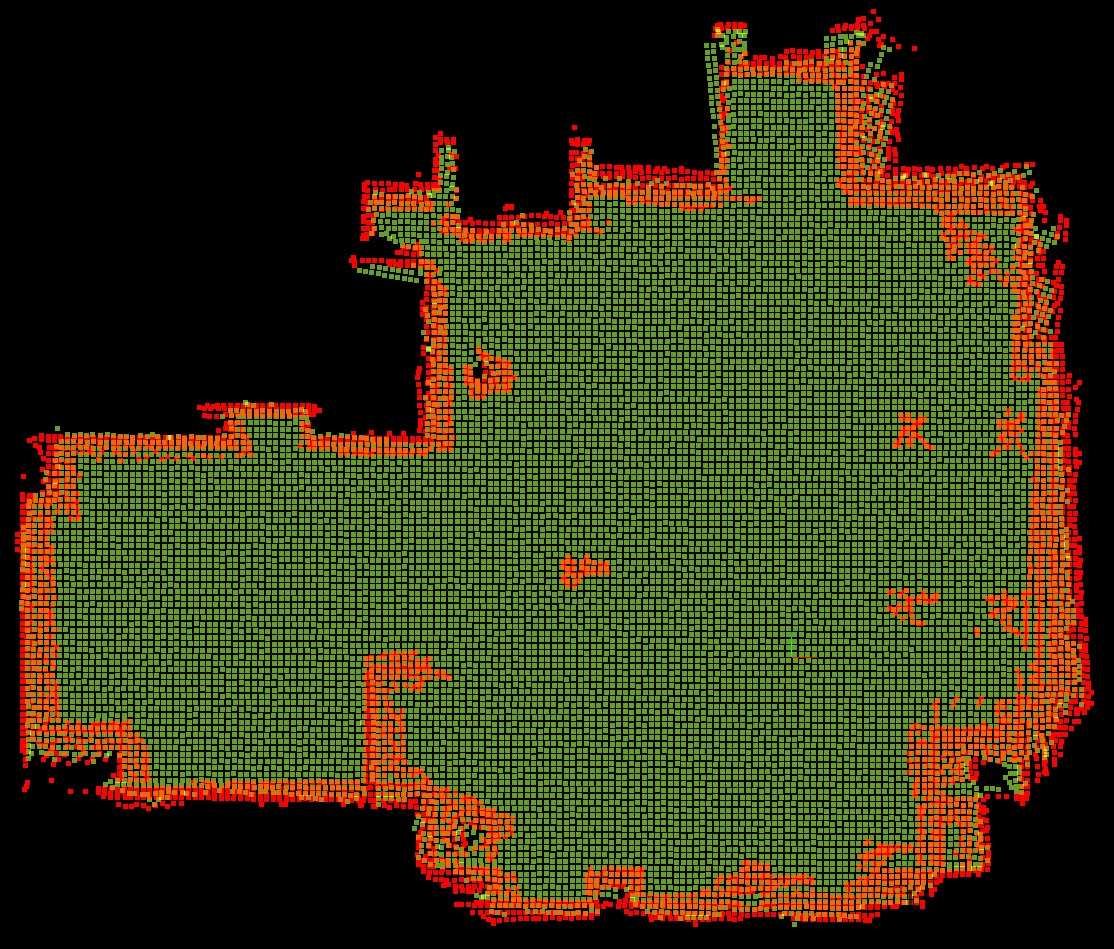
\includegraphics[width=.7\linewidth]{my_world_og.png}
  \caption{Occupancy Grid - My World}
  \label{fig:my-og}
\end{figure}


Both environments had several features that could beused to detect global loop closures. Figure \ref{fig:loopclosure} shows the camera frames where loop closures were detected. The circles marked in pink indicates where two images have features in common.

\begin{figure}[H]
\centering
\begin{subfigure}{.5\linewidth}
  \centering
  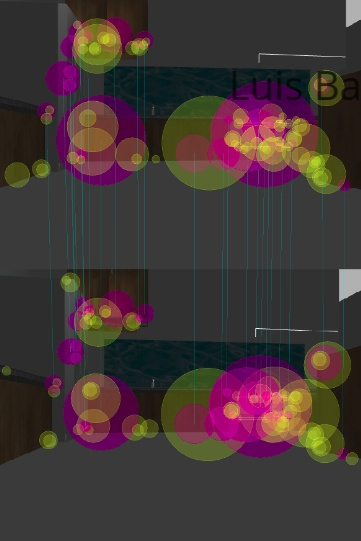
\includegraphics[width=.95\linewidth]{kd_world_loop_closure.png}
  \caption{Kitchen and Dining World}
  \label{fig:kd-loopclosure}
\end{subfigure}%
\begin{subfigure}{.5\linewidth}
  \centering
  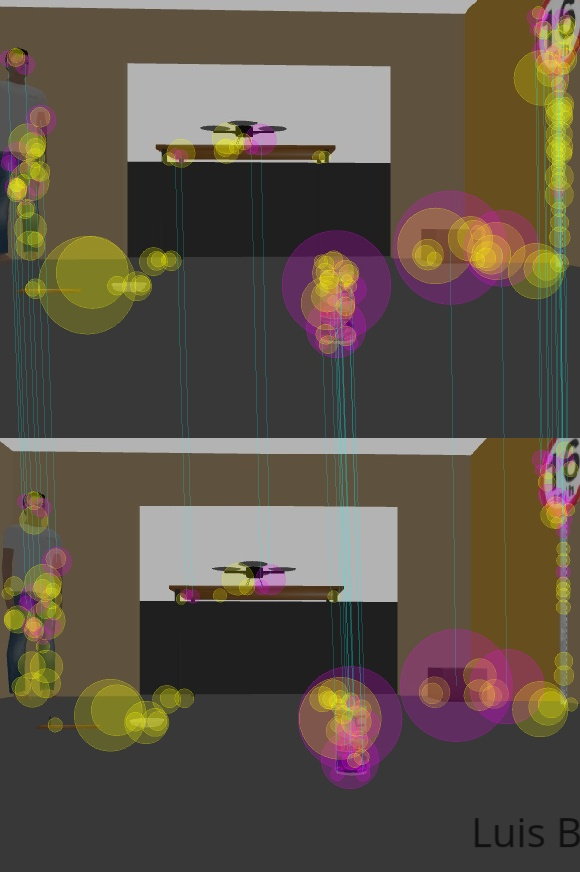
\includegraphics[width=.95\linewidth]{my_world_loop_closure.png}
  \caption{My World}
  \label{fig:my-loopclosure}
\end{subfigure}
\caption{Loop Closure}
\label{fig:loopclosure}
\end{figure}

Figures \ref{fig:kd-3d} and \ref{fig:my-3d} shows the final point cloud generated by the RGB-D sensor. In both environments, it is possible to observe good fidelity comparing with the original map. Several items, such as tables, chair, boxes, and others, can be recognized as well.
It is also possible to notice that the density of the point cloud depends on how many times the robot was driven by the area. In some places where the robot did not go very often, the density of the point cloud is lower.

\begin{figure}[H]
\centering
  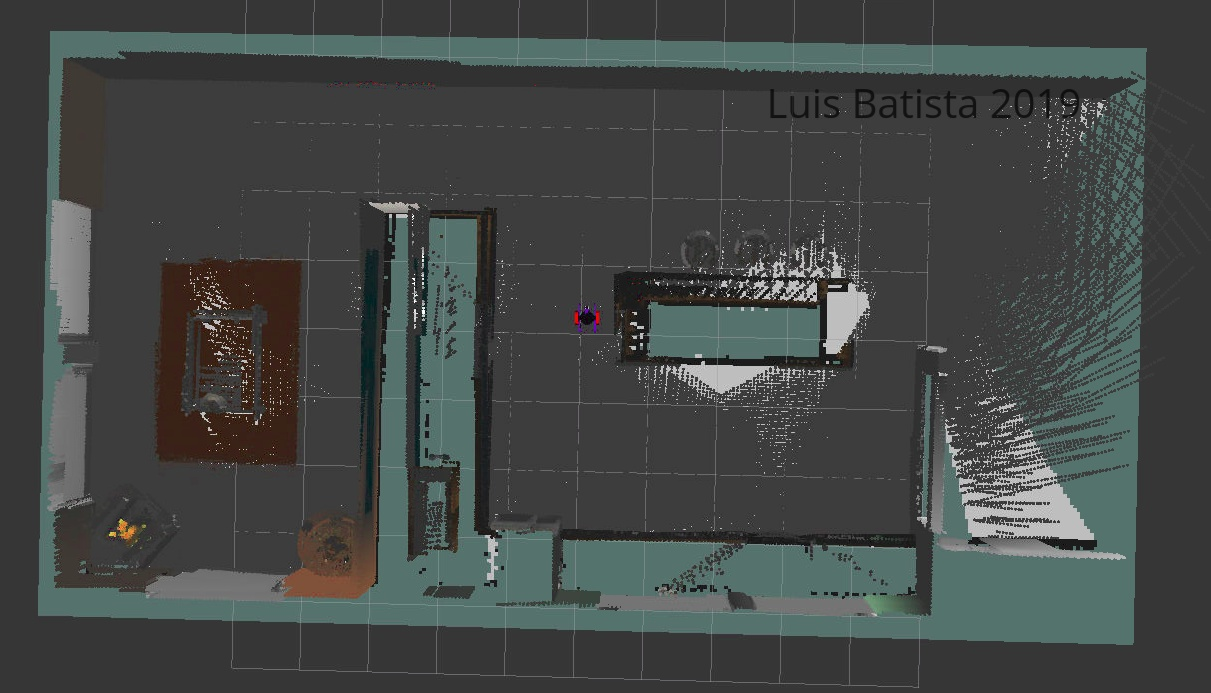
\includegraphics[width=.9\linewidth]{kd_world_3d.png}
  \caption{3D Map - Kitchen and Dining World}
  \label{fig:kd-3d}
\end{figure}%

\begin{figure}[H]
\centering
  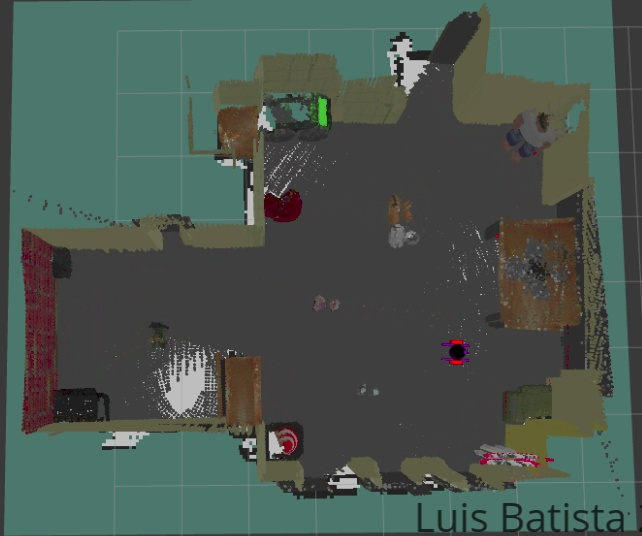
\includegraphics[width=.7\linewidth]{my_world_3d.png}
  \caption{3D Map - My World}
  \label{fig:my-3d}
\end{figure}



\section{Discussion}

In both cases, the generated map was very close to the original simulated environment. By carefully inspecting the occupancy grid and the final point cloud, it is possible to verify that the Kitchen and Dining map had a more precise and sharp result. It is worth mentioning the different computer were used in each case. While the My World was mapped in a personal computer, the Kitchen and Dining world was mapped in the workspace provided by Udacity.

During initial mapping tests, some objects were not static. As the position of the object slightly changed over time, the loop closure algorithm had lower quality results. In order to achieve better results, it was necessary to guarantee that no object was moving during each lap of the robot. 

For plain maps without many visual features, it was observed several incorrect loop closures. Eventual false correlation of different locations created a significant distortion of the map. This was solved by deliberately placing unique objects around the environment. 

It was also observed that the placement of the lidar is important as the occupancy grid will reflect the objects detected by that sensor. Note that smaller objects, such as the Hummer located on the floor of the My World, is not considered in the occupancy grid. Nevertheless, it is useful to increase the image features used for loop detection.



\section{Future work}

The first step would be to apply the mapping algorithm in real robots. This will allow to test performance on real hardware and very how the RTAB-Map can perform data association with actual images that are much more feature rich when compared to a simulated environment.

The next step would be to extend the robot including additional sensors. By implementing a proper sensor fusion of the data, it is expected to reduce the uncertainties in the SLAM results based on the sensor errors. 

One additional customization to be considered is the investigate options to perform SLAM that is tolerant to a dynamic environment with moving objects. This would have a strong impact on the loop closure approach using in this project but is extremely important in real-world applications.

%\bibliography{bib}
%\bibliographystyle{ieeetr}

\end{document}
